\documentclass[titlepage,12pt,a4paper]{article}

\usepackage[left=2cm,top=3cm,right=2cm,bottom=3cm,bindingoffset=0.5cm]{geometry}
\usepackage{amsmath}
\usepackage{amssymb}
\usepackage{enumitem}
\usepackage{commath}
\usepackage{mathtools}
\usepackage{graphicx}
\usepackage{csquotes}
%\usepackage{dirtytalk}
\usepackage{hyperref}
\usepackage{tabto}
\usepackage{gensymb}
\usepackage{graphicx}
\usepackage{listings}
\usepackage{sidecap}
\usepackage{wrapfig}
\usepackage{parskip}

\usepackage{fancyhdr}
\usepackage{color}
\definecolor{dkgreen}{rgb}{0,0.6,0}
\definecolor{gray}{rgb}{0.5,0.5,0.5}
\definecolor{mauve}{rgb}{0.58,0,0.82}

\lstset{frame=tb,
  language=C++,
  aboveskip=3mm,
  belowskip=3mm,
  showstringspaces=false,
  columns=flexible,
  basicstyle={\small\ttfamily},
  numbers=left,
  numberstyle=\footnotesize,
  stepnumber=1,
  numbersep=5pt,
  keywordstyle=\color{blue},
  commentstyle=\color{dkgreen},
  stringstyle=\color{mauve},
  breaklines=true,
  breakatwhitespace=true,
  tabsize=3
}


\pagestyle{fancy}\lhead{A} \rhead{C}
\chead{{\large{\bf B}}}
\lfoot{}
\rfoot{\bf \thepage}
\cfoot{}

\setlength{\headheight}{15.2pt}
\pagestyle{fancy}
\fancyhf{}
\lhead{ \fancyplain{}{COMP3431: Robotic Software Architecture} }
\rfoot{ \fancyplain{}{\thepage} }


\begin{document}
\begin{titlepage}
    \begin{center}
        \vspace*{3cm}
        
        \Huge
        \textbf{COMP3431\\}
        \title{}
        \vspace{0.5cm}
        \Huge
        \textbf{Robotic Software Architecture}
        
        \vspace{0.54cm}
        
        \Large
        Assignment 2: Report
        
        \vspace{5cm}

	\large
	Nathan ADLER\\
	Aneita YANG\\

	\vfill
        
        \Large
        November 9, 2015
        
    \end{center}
\end{titlepage}

\pagebreak
\tableofcontents

\pagebreak
\section{Introduction}
In this assignment, both the hardware and software aspects of robotics were explored. The overall objective was to create a robot that would drive autonomously in an outdoor environment, whilst avoiding any obstacles. A motorised wheelchair was the baseline from which the robot was constructed.

To achieve the objective, the robot is equipped with a GPS and compass (using an Android phone with ROS). A laser scanner is also attached to the front of the robot, gathering information about the robot's immediate surroundings.

\subsection{Modules}
Five modules run in conjunction to operate the robot.

\pagebreak
\section{Hardware}
\begin{itemize}
	\item Dell Latitude E6400 notebook
	\item SICK TiM551 2D laser scanner
	\item DLink DSL 2750B N300 Modem Router
	\item Sony Xperia Z3 compact
	\item Arduino Mega 2560 R3
	\item Sabertooth 2X25 regenerative motor driver
	\item 2 x 12V lead acid battery
	\item 2 x electric wheelchair motor
\end{itemize}

\begin{figure}
	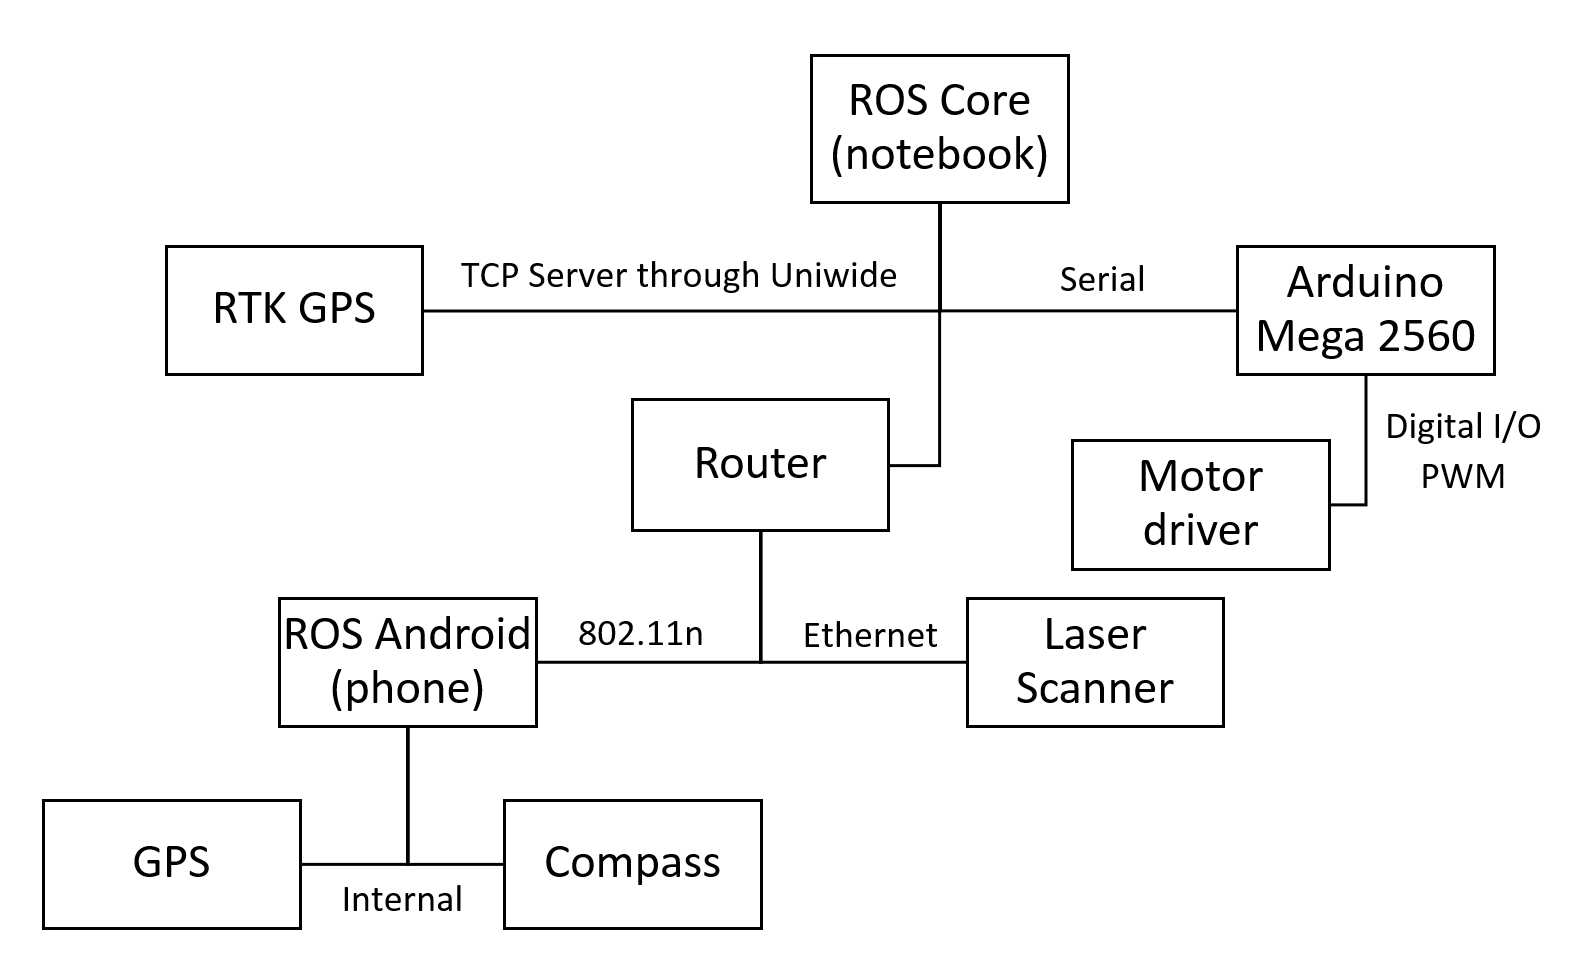
\includegraphics[scale=0.8]{figures/hardware_chart.png}
	\caption{Hardware map of UGV}
	\label{figure:hardware_chart}
\end{figure}

\pagebreak
\section{Software}

\pagebreak
\section{Results}

\pagebreak
\section{Future Work and Improvements}

\pagebreak
\section{Appendix}

\end{document}
